\documentclass[a4paper,10pt]{article}
\usepackage{graphicx}
\usepackage{fullpage}
\usepackage{fancyhdr}
\usepackage{fourier}
\usepackage{framed}
\usepackage{booktabs}
\usepackage[hyphens]{url}
\usepackage{hyperref}
\usepackage{array}
\usepackage[justification=justified,singlelinecheck=false]{caption}
\usepackage{float}
\usepackage{todonotes}
\usepackage{subcaption}
\usepackage{natbib}
\usepackage{tocloft}
\usepackage{todonotes}

\setlength{\cftbeforesecskip}{6pt}
\setlength{\headsep}{20pt}
\setlength{\headheight}{12pt}
\pagestyle{fancy}
\setlength{\parskip}{10pt plus 1pt minus 1pt}
\sloppy

\newenvironment{tight_enumerate}{
\begin{enumerate}
  \setlength{\itemsep}{0pt}
  \setlength{\parskip}{0pt}
}{\end{enumerate}}

\newenvironment{tight_itemize}{
\begin{itemize}
  \setlength{\itemsep}{0pt}
  \setlength{\parskip}{0pt}
}{\end{itemize}}

\newcommand{\para}[1]{\paragraph{#1}\mbox{}\\}

\begin{document}
\begin{titlepage}
\begin{center}
  \bfseries
  \huge SCalable Metagenomics Pipeline (SCaMP) \\User Guide
  \vskip 0.1in
  \textsc{\normalsize Version 0.10 }
  \vskip 0.1in
  \textsc{\normalsize James Abbott (j.abbott@imperial.ac.uk)}
\end{center}

\tableofcontents
\renewcommand{\baselinestretch}{1.0}\normalsize
\end{titlepage}
\newpage
\graphicspath{ {images/} }

\section{Introduction}

The SCalable Metagenomics Pipeline (SCaMP) is a system for high-throughput
analysis of shotgun metagenome samples. It combines many tools (selected as
being the most effective in our evaluations) to determine community
composition, gene representation and abundance through metagenome assembly and
annotation and pathway representation. 

\section{Installation}

SCaMP requires a number of prerequisite packages to be installed, in addition                            
to the SCaMP software itself. This can either be achieved by installing all the
required packages and Perl modules manually, or through the use of conda, which
is the recommended approach since it greatly simplifies installation.  

\subsection{Quick installation with Conda (Recommended)}

You will need to first install both git and miniconda, and setup conda channels
as described on the bioconda installation page: \url{https://bioconda.github.io/#install-conda}.                                  

\subsubsection{SCaMP installation}

SCaMP can be then be downloaded from the git repository using the command:                                           

{\tt git clone https://github.com/jamesabbott/SCaMP.git}

Once the repository is cloned, the prerequisite packages can be installed from
conda using the {\tt setup.sh} script:           

{\tt SCaMP/bin/setup.sh}

The setup script will create a new conda environment name 'SCaMP' to avoid
conflicts with any existing conda installations, and use this to install
the prerequisite packages. Once completed, the script will give the option of
appending the SCaMP bin directory to your path. This will ensure the SCaMP
commands are readily available from the command line.

\subsubsection{Customising the SCaMP Environment}

If your system requires specific configuration such as manually setting a path,
or loading an environment module to access conda, then the {\tt bin/SCaMP}
script can be edited to include any necessary settings. See the comments at the
top of the script for examples of the kind of configuration which may be
configured. The {\tt setup.sh} script will have uncommented a line in this
section to activate the SCaMP conda environment each time the software is run.

\subsection{Manual Installation (The Slow Way...)}

% comment out conda lines in SCaMP
\subsubsection{Perl Modules}

A number of non-standard perl modules need to be installed prior to installing SCaMP: 

\begin{tight_enumerate}
\item BioPerl                                          
\item Bio::DB::EUtilities                              
\item DateTime                                         
\item File::Copy::Recursive                            
\item File::Find::Rule                                 
\item HTML::Entities                                   
\item LWP                                              
\item LWP::Protocol::https                             
\item Net::FTP::Recursive                              
\item Parallel::ForkManager                           
\item XML::Simple                                     
\item YAML::XS            
\end{tight_enumerate}

Most of these will be available through your systems package management system
(using {\tt yum} or {\tt apt}), however others may require installation from
CPAN.  

\subsubsection{Prerequisite packages}

A number of software packages also need to installed, and made available on the
system path prior to running SCaMP. These are listed in table
\ref{tab:reqpack}, along with tested version numbers.

\begin{table}[htb]
\begin{tabular}{lll}
\hline
\textbf {Package} & \textbf {Tested Version}  & \textbf{Download Site} \\
\hline
bwa		& 	0.7.15 	&	http://bio-bwa.sourceforge.net	\\               
cutadapt	&	1.15	&	https://github.com/marcelm/cutadapt \\	
FastQC		& 	0.11.5 	&	https://www.bioinformatics.babraham.ac.uk/projects/fastqc	\\
picard		& 	2.15.0 	&	http://broadinstitute.github.io/picard	\\
R		& 	3.3.2 	&	http://r-project.org	\\	
samtools	& 	1.3.1 	&	http://www.htslib.org	\\
trim-galore	& 	0.45	& 	https://www.bioinformatics.babraham.ac.uk/projects/trim\_galore	\\
\hline
\end{tabular}
\captionof{table}{Required software packages}
\label{tab:reqpack}
\end{table}

\subsubsection{SCaMP installation}

SCaMP can be now be downloaded from the git repository using the command:                                           

{\tt git clone https://github.com/jamesabbott/SCaMP.git}

\subsubsection{Customising the SCaMP Environment}

If your system requires specific configuration such as manually setting a path,
or loading an environment module to access conda, then the {\tt bin/SCaMP}
script can be edited to include any necessary settings. See the comments at the
top of the script for examples of the kind of configuration which may be
configured.

\section{About SCaMP}

\subsection{The Pipeline} \label{pipeline}

The SCaMP workflow consists of a number of independent stages
(Figure \ref{fig:scamp_workflow}), and is designed to be run under a batch-queuing
environment (PBSPro or Sun Grid Engine). A work directory needs to be created
on shared storage accessible by the compute nodes under the control of the
queueing system, and fastq files copied into a {\tt reads} directory within
this work directory. Depending upon the compute configuration, data can either
be copied to local storage on compute nodes, or analysed directly within the
work directory. The path to the work directory needs to be defined within a
SCaMP.yaml configuration file. Output files will be written within the work
directory as the various stages of the pipeline are run. The stages of the
SCaMP workflow need to be executed in the correct order - stages will look for
the outputs files of preceding stages in the workflow as their input files,
consequently executing the stages out of sequence will result in failed jobs. A
summary of the various stages and execution order is shown in table
\ref{tab:scamp_stages}. 

\begin{figure}[!h] \fbox{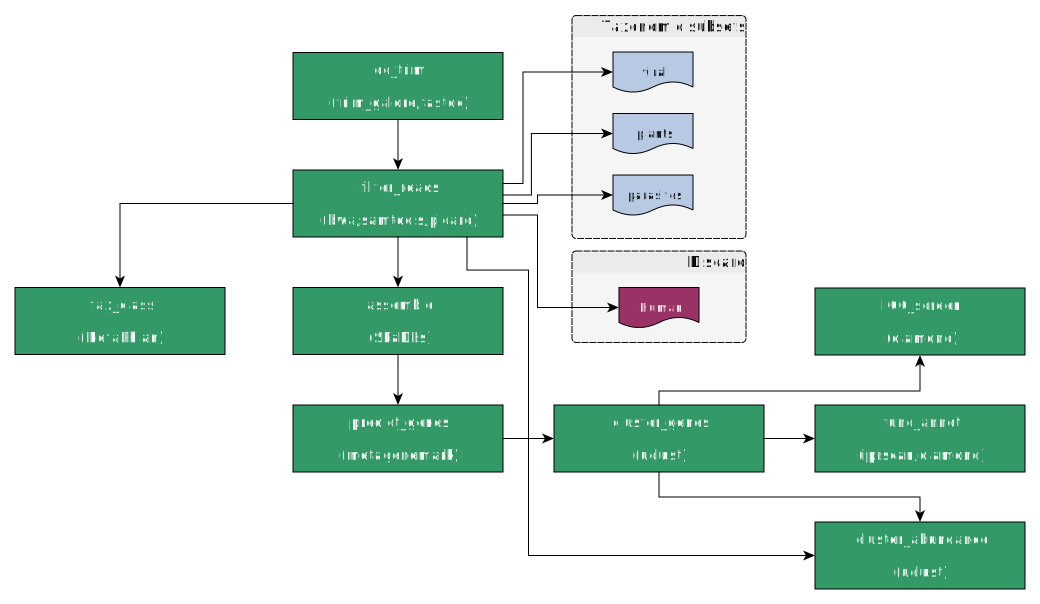
\includegraphics[width=0.9\textwidth]{SCaMP_workflow}}
\caption{SCaMP Workflow} \label{fig:scamp_workflow} \end{figure}

\begin{table}[htb]
\begin{tabular}{lll}
\hline
\textbf {Stage} & \textbf {Order}  & \textbf{Summary} \\
\hline
qc\_trim			& 	1 	&	Carries out QC analysis of sequence reads, and trims low-quality sequence and adapters \\
filter\_reads 	&	2	&	Filters reads against databases of known sequences to remove e.g. host contaminants \\
\hline
\end{tabular}
\captionof{table}{Stages of the SCaMP workflow, including execution order.}
\label{tab:scamp_stages}
\end{table}

\subsection{Software Layout}

The SCaMP software is laid out across a few directories, the contents of which
are hopefully self-explanatory:

{\tt bin} - Executable scripts:
\begin{tight_itemize}
\item \textbf{build\_ref\_db}: Downloads and indexes reference databases.
\item \textbf{filter\_reads}: Filters sequence reads against reference database.
\item \textbf{qc\_trim}: Runs QC on sequence reads and applies quality and adapter trimming.
\item \textbf{SCaMP}: Main script for launching analysis runs.
\item \textbf{setup.sh}: Installs prerequisite packages and configures system.
\end{tight_itemize}

{\tt doc} - Documentation
\begin{tight_itemize}
\item \textbf{SCaMP\_User\_Guide.tex}: LaTeX source for user guide.
\item \textbf{SCaMP\_User\_Guide.pdf}: PDF format user guide.
\end{tight_itemize}

{\tt etc} - Configuration data
\begin{tight_itemize}
\item \textbf{barcodes.txt}: Example barcode sequences for adapter trimming.
\item \textbf{conda\_packages.txt}: List of conda packages to be installed by {\tt bin/setup.sh}.
\item \textbf{SCaMP.yaml}: YAML format configuration file.
\end{tight_itemize}

{\tt lib} - Common software components used by scripts in {\tt bin}
\begin{tight_itemize}
\item \textbf{SCaMP.pm}: Class of common methods used by scripts in {\tt bin}.
\end{tight_itemize}

\subsection{Preparing to Run SCaMP}

\subsubsection{Configuration File}

The {\tt etc/SCaMP.yaml} defines the SCaMP configuration. In shared
installations, each user can copy this file to a file named {\tt .SCaMP.yaml}
in their home directory. If this file is found, then the configuration will be
read from this file in preference to the {\tt etc/SCaMP.yaml} file.

The configuration file should be edited to define the following attributes:

\begin{tight_itemize}
\item \textbf{work\_dir}: Path to directory where SCaMP analysis will be carried out
\item \textbf{database\_dir}: Path to directory for storing reference databases
\end{tight_itemize}

A series of directories will be created in {\tt work\_dir} as the analysis
proceeds, storing various intermediate files and analysis results. 

In a shared software installation, a single set of reference databases can be
downloaded and stored in a centralised {\tt database\_dir} to reduce disk space
usage. 

\subsubsection{Sequence Reads}

A directory should be created in {\tt work\_dir} named {\tt reads}, and fastq
files (preferably compressed using gzip) for the project should be copied into
this directory.

SCaMP is designed to be run using paired reads from an Illumina sequencer,
typically a MiSeq or HiSeq. In order for the reads to be identified correctly
they should be named in accordance with one of the following convention:

\textit{samplename(\_barcode)?(\_xxxxx)?\_R[12].f(ast)?q.gz}

The filename should start with the name of the sample, followed by an optional
barcode (typically six or eight bases). Additional details may optionally be
included in the next section of the filename, following which the filename must
include either \_1/\_2, or \_R1/\_R2 (indicating read 1 or read 2 of the paired
reads). The filename should be suffixed with either .fastq.gz or fq.gz.

Examples of valid filenames include:
\begin{tight_itemize}
\item \textit{Sample-001\_R1.fastq.gz}
\item \textit{Sample-002\_R2.fq.gz}
\item \textit{Sample-003\_12.fq.gz}
\item \textit{Sample-004\_TAATCG\_L005.R1.fastq.gz}
\end{tight_itemize}

\subsubsection{Reference Databases}

SCaMP allows samples to be filtered against various taxonomic databases to
remove e.g. host contamination. The databases should be located within the
directory specified by the {\tt database\_dir} parameter in the {\tt SCaMP.yaml}
configuration file. A separate subdirectory should be created for each database
(named with the database name), and within this multiple copies of the database
can exist in e.g. time-stamped directories, with a symlink named 'latest' to
the most recent copy of the database, which will be used for analysis.

\para{Reference Database Format}

Each database used by for filtering by these scripts requires the following:

\begin{tight_enumerate}
\item A fasta formatted sequence of sequences, named 'database.fa'
\item A fasta index, generated with 'samtools faidx' ('database.fa.fai')
\item BWA indices appropriate for searching with BWA MEM 
\item A tab-delimited file ('database.tax.dat') relating taxonomy data to each sequence ('database.taxid.dat')
\end{tight_enumerate}

The tab-delimited file should be formatted as follows:

\begin{verbatim}
##Accession   Scientific name  Strain  NCBI TaxId
chr1    Homo sapiens            9606
578454_CABE01000000     Candida parapsilosis    CDC317  578454
\end{verbatim}

In the Homo sapiens example there is no strain defined, so this field is simply left blank

\para{Downloading Databases}

The {\tt bin/build\_ref\_db} script allows preconfigured reference databases to
be downloaded and appropriately formatted, with the resulting databases being
made available in {\tt database\_dir}. A list of the databases available for
downloaded can be obtained by running

{\tt build\_ref\_db --avail}

Downloading and formatting a database can be achieved by running

{\tt build\_ref\_db --db dbname}

\para{Database Configuration}

Configurations for the available databases are defined in the {\tt databases}
block of the SCaMP configuration file. These can be modified as required to
create custom databases for screening sequence reads. The following parameters
may be defined to configure a database:

\begin{tight_itemize}
\item \textbf{format}: Format of reference database. Valid values: embl/genbank
\item \textbf{type}: Download type. Valid values: ftp/entrez/entrez\_accession.
\begin{tight_itemize}
\item \textit{ftp}: Defines a database to be downloaded from an ftp server.
Requires \textit{ftphost}, \textit{ftpdir} and \textit{filepattern} parameters
to be defined.
\item \textit{entrez}: Defines a database to be retrieved from the NCBI using
an entrez query. Requires \textit{entrez\_query} parameter to be defined.
\item \textit{entrez\_accession}: Defines a database to be retrieved from the
NCBI using entrez from a list of accessions. Requires \textit{accession}
parameter to be defined.
\end{tight_itemize}
\item \textbf{ftphost}: URI of FTP server i.e. {\tt ftp.ensemblgenomes.org}
\item \textbf{ftpdir}: Path to directory on FTP server where database is found.
i.e.  {\tt /pub/plants/current/embl}
\item \textbf{filepattern}: Regular expression defining list of files to be
downloaded. i.e. {\tt .dat.gz\$}
\item \textbf{entrez\_query}:  Entrez query to select records for inclusion in
database i.e. {\tt "Viruses"[Organism]}
\item \textbf{accessions}: List of accession to be included in database
\end{tight_itemize}

\section{Running SCaMP}

SCaMP is designed to be run under either a PBSPro or Sun Grid Engine
batch-queueing environment. While all the components of the pipeline can be
submitted manually, the {\tt SCaMP} script will take care of submitting the
correct number of array tasks to the available queueing system. 

Each component (or stage) or the pipeline is run by a separate script located
in the {\tt bin} directory.  SCaMP requires the stage of the pipeline to run to
be defined, and will pass through additional command-line arguments to the
individual stage script. Provided arguments will be verified before the jobs is
submitted to the queueing system.

Running {\tt SCaMP} without any arguments provides usage information, along
with a list of the available stages which can be run. \textbf{N.B. stages must
be executed in the correct order, as described below.}

\todo{Update output\ldots}
\begin{verbatim}
[jamesa@wssb-james ]$ SCaMP 

SCaMP: SCalable Metagenomics Pipeline
usage: /home/jamesa/src/SCaMP/bin/SCaMP -r run_stage [-l|--local] [-- script arguments]

Configured stages: qc_trim filter_reads

[jamesa@wssb-james doc]$ 
\end{verbatim}

SCaMP is designed to be run either on cluster environments with local storage
available on each compute node, or on systems with high-performance parallel
filesystems i.e. GPFS/Lustre. In a typical cluster environment, it is
preferable for data to be copied to a temporary directory on the execution node
to ensure heavy IO loads take place on faster local storage and reduce network
load on the cluster. In contrast, systems with parallel file systems or large
shared memory machines with locally attached storage can manage the IO loads
from shared storage adequately, hence it is optimal not to move data to a
temporary directory for computation.

By default, SCaMP will copy databases and sample data to a temporary directory
on each cluster node. If your environment benefits from fast shared storage,
then SCaMP can be run using the {\tt -l} or {\tt --local} arguments, in which
case the databases and sample data will not be copied to local temporary
directories. For example, the command:

\begin{verbatim}
SCaMP -r qc_trim --local
\end{verbatim}

will execute the 'qc\_trim' stage using local storage. Consult your local
system maintainers if you are unsure of whether local storage or temporary
storage on the compute nodes should be used in your environment. 

Executing the 'SCaMP' script results in the command-line parameters being
validated by the stage script, to ensure that all necessary arguments have been
provided, and that the directories/files required for the stage to run are
available prior to submitting the job. Once these have been validated
successfully, the  job will be submitted to the PBS or SGE system and the job
id of the stage will be displayed on the screen. Progress of the job can then
be monitored using the {\tt qstat} command. 

Once the job completes, any standard output or standard error generated during
it's execution will be writen to a file named {\tt SCaMP:stage.oJOBID.TASKID}
in the directory from which the job was submitted.

\subsection{SCaMP Stages}

The following section descriptions obtained from the embedded help
documentation within each script. Please refer to \ref{pipeline} for the
correct ordering in which the stages should be run.

\include{stages/qc_trim}
\include{stages/filter_reads}

\subsection{Example Analysis}

The following commands illustrate a typical run of the SCaMP pipeline in the correct order of execution.

\begin{verbatim}
SCaMP -r qc_trim
SCaMP -r filter_reads --db human
SCaMP -r filter_reads --db plants 
SCaMP -r filter_reads --db fungi
SCaMP -r filter_reads --db parasites
\end{verbatim}

\end{document}
